\documentclass[a4paper, 11pt]{report}


%────────────────────────────────────────────────────────────────────────────────────────────────────────────────────────────────────────────────────
%
%   PACKAGES
%
%────────────────────────────────────────────────────────────────────────────────────────────────────────────────────────────────────────────────────

\usepackage{microtype}
\usepackage{hyperref}
\usepackage[dvipsnames,table]{xcolor}
% remove the outline of the links

\hypersetup{
    colorlinks,
    linkcolor={black},
    citecolor={black},
    urlcolor={black}
}

\usepackage[scale=0.70]{geometry}
\usepackage{graphicx}
\usepackage{lipsum}

\mathchardef\mhyphen="2D


\usepackage[utf8]{inputenc} % Required for inputting international characters
\usepackage[T1]{fontenc} % Output font encoding for international characters

\usepackage{kpfonts,baskervald}

\usepackage{parskip}
\usepackage{tcolorbox}

\usepackage{subfig}
\usepackage{float}

\newtcolorbox{basecolorbox}[1][]{%
  colback=gray!25, colframe=gray!25,
  coltitle=black, fonttitle=\Large\bfseries,
  rounded corners,
  width = (\linewidth-30pt),
  title=#1}

\newenvironment{titlebox}[1][]{%
  \centering
  \basecolorbox[#1]%
}{%
  \endbasecolorbox%
}

\newenvironment{inlinebox}[1][]{%
  \titlebox%
  {\upshape\bfseries #1}%
}{%
  \endbasecolorbox%
}


\usepackage{cleveref}

\author{Martina Doku \and Giuseppina Iannotti \and Dennis Locatelli \and Elena Muià \and Dario Loi \and Davide Marincione}

\title{\Huge Report for HCI} % to be changed

\begin{document}

\begin{titlepage} % Suppresses displaying the page number on the title page and the subsequent page counts as page 1
	\newcommand{\HRule}{\rule{\linewidth}{0.5mm}} % Defines a new command for horizontal lines, change thickness here

	\center% Centre everything on the page

	%------------------------------------------------
	%   Headings
	%------------------------------------------------

	\textsc{\LARGE Sapienza University of Rome}\\[1.5cm] % Main heading such as the name of your university/college

	\textsc{\Large Human Computer Interaction -- A.Y 2022/2023}\\[0.5cm] % Major heading such as course name

	\textsc{\large Applied Computer Science and Artificial Intelligence}\\[0.5cm] % Minor heading such as course title

	%------------------------------------------------
	%   Title
	%------------------------------------------------

	\HRule\\[0.4cm]

	{\huge\bfseries A Crowd-Sourced Mobility Application}\\[0.4cm] % Title of your document

	\HRule\\[1.5cm]

	%------------------------------------------------
	%   Author(s)
	%------------------------------------------------

	\begin{minipage}{0.4\textwidth}
		\begin{flushleft}
			\Large
			\textit{Authors:}\\[3pt]\hspace{2pt} % insert a 2pt indentation
			Doku \textsc{Martina}\\[1pt]\hspace{2pt}
			Iannotti \textsc{Giuseppina}\\[1pt]\hspace{2pt}
			Locatelli \textsc{Dennis}\\[1pt]\hspace{2pt}
			Muià \textsc{Elena Maria}\\[1pt]\hspace{2pt}
			Loi \textsc{Dario}\\[1pt]\hspace{2pt}
			Marincione \textsc{Davide}
		\end{flushleft}
	\end{minipage}
	\begin{minipage}{0.4\textwidth}
		\begin{flushright}
		\end{flushright}
	\end{minipage}

	% If you don't want a supervisor, uncomment the two lines below and comment the code above
	%{\large\textit{Author}}\\
	%John \textsc{Smith} % Your name

	%------------------------------------------------
	%   Date
	%------------------------------------------------

	\vfill\vfill\vfill % Position the date 3/4 down the remaining page

	{\large May 2, 2023} % Date, change the \today to a set date if you want to be precise

	%------------------------------------------------
	%   Logo
	%------------------------------------------------

	%\vfill\vfill
	%\includegraphics[width=0.2\textwidth]{placeholder.jpg}\\[1cm] % Include a department/university logo - this will require the graphicx package

	%----------------------------------------------------------------------------------------

	\vfill % Push the date up 1/4 of the remaining page

\end{titlepage}

\tableofcontents

\chapter{Introduction}
%Decide if we want to scale back to section, find a way to
% suppress the numbering of the chapter so that first section is
% 1.0 and not 0.1
\section{Our Idea}\label{sec:our-idea}
The intent of our application is to give more precise information about possible delays or irregularities in the public transportation service. This could be achieved by the retrieval of information delivered directly by the community of users, who may have the chance to inform others about possible delays or overcrowding of the bus or the tram that they are taking.
Furthermore, all the users will collect some credits for every contribution, which will be devolved into charity, in one of the NGOs chosen by the user, among those proposed by the application.

\section{Existing Competitors}\label{sec:existing-competitors}

\paragraph{Google Maps:} It is one of Italy's most frequently used mobility applications. It is a web service that provides detailed information about geographical regions and sites worldwide. In addition to conventional road maps, Google Maps offers aerial and satellite views of many locations. It works both for public transportation and private ones.
\begin{itemize}
	\item \textbf{Pros:} It is very intuitive and offers many fundamental features. It delivers information about possible paths to reach the destination with their duration and arrival time. It specifies the possible expenses needed for every choice taken.
	\item \textbf{Cons:} The path duration is not defined by crowdsourced information or GPS tracking applications. It is based totally on statistical inferences which means that is almost never precise.
\end{itemize}

\paragraph{Moovit:}  It is one of the main mobility applications for public transportation only. It provides information about the statistically best path to reach a destination point. Describing when and where to take the transportation means in order to reach the destination as fast as possible.

\begin{itemize}
	\item \textbf{Pros:} More reliable than Google Maps (based on users' interviews), the interface is very intuitive.
	\item \textbf{Cons:} Too many ads, the defined timing is almost never correct.
\end{itemize}

\paragraph{Probus:}The application is designed for Android only and it only works with buses. It informs the user about the waiting time of a certain bus line and the fastest path to reach a destination.

\begin{itemize}
	\item \textbf{Pros:} Useful because it is strictly focused on busses, and therefore is able to offer a more tailored experience to users.
	\item \textbf{Cons:} Although the time estimates are reliable within a single bus trip, the application does \emph{not} give information about future ones, hence, users do not know how long they will have to wait for the next run.
\end{itemize}

\paragraph{Citymapper:} Citymapper is a public transit app and mapping service which displays transport options, usually with live timing, between any two locations in a supported city. It integrates data for all urban modes of transport, including walking, cycling, and driving, in addition to public transport.

\begin{itemize}
	\item \textbf{Pros:} An almost always accurate and comprehensive direction guide. Free for both Android and iOS.\@ It provides a calories counter and 	specifies the expenses for every chosen path.
	\item \textbf{Cons:} Not available in many cities and it does not retrive crowdsourced information.
\end{itemize}

\paragraph{Transit:}  Transit is a mobile app packed with features that help you plan a trip on the bus. Real-time bus tracking and information, service alerts, and trip planners are some of the many useful features that make this app a favorite for transportation services.

\begin{itemize}
	\item \textbf{Pros:} GPS tracking of public transportation in real-time, crowdsource support (tracking the user location when they use the app as a navigator), information about all the surrounding bus stops and possible paths to the destination.
	\item \textbf{Cons:} Many useful services are not free.\@ It does not work very well in Italy.
\end{itemize}

\section{Need Finding}\label{sec:need-finding}

\subsection{The Interviews}\label{ssec:the-interviews}

In order to better understand what our users want, we first conducted a round of interviews.
These allowed us to interact colloquially with our potential users and to gauge what they think
are the major discomforts of public transportation. We also wanted to understand their approach
to personal privacy and community-driven applications. We used data we obtained as a guide for our
next steps in the design process.

\paragraph{Our Questions}

Our interviews were standardized around a set of ten questions that we designed, as a group,
to be as open-ended as possible. We wanted to avoid leading the interviewees to answer in a
particular way, have them act as designers, or figure out the specific purpose of the
survey until later on, when the general questions were answered.\\[2pt]

\begin{titlebox}[The Questions:]
	\begin{enumerate}
		\item Did you commute via public transport in the last week? If so, what type?
		\item What criteria do you consider when choosing your means of transportation?
		\item What are some frustrating aspects about public transportation?
		\item Do you use mobility apps (like Google Maps) while commuting? If so, which
		      functionalities?
		\item How much do you trust the information given by your app of choice?
		\item Do you worry about giving authorizations to apps? Are there some you are more willing to share?
		\item Are you concerned about organizations distributing your location based data to third parties?
		\item Would you trust mobility info more if it were crowd-sourced? Would you participate
		      in such a program?
		\item Would a honor system, rewarding you based on the credibility of
		      your contributions, incentivize you to participate more?
		\item In a community-driven app, how interested are you in customizing and showing your
		      profile?
	\end{enumerate}
\end{titlebox}

\paragraph{The Outcomes}

To carry out the interviews, we split our groups into 3 teams of 2 people each. Each of those
teams had a target of 10 interviews to reach, which was achieved in a few days (with
some extra interviews to spare).

Overall, if we look at the general trends, we can draw the following conclusions:

\begin{itemize}
	\item A majority of our interviewees use public transportation on a daily basis, and most of
	      them commute via bus or metro.
	\item All of the interviewees use mobility apps, with Google Maps being the most popular,
	      usually paired with an app such as Moovit to provide more accurate information.
	\item Most of the interviewees find frustration in three things:
	      \begin{enumerate}
		      \item Overcrowding of the vehicles
		      \item Lack of punctuality
		      \item Unreliability of bus rides (which are often late or do not show up at all)
	      \end{enumerate}
	\item Users are generally willing to share data that is required for the functioning of the app,
	      and are only really concerned about their privacy if the issue is brought up.
	\item Users enjoy the prospect of a community-driven application, and would be willing to
	      participate in such a program, especially if it were to improve the quality of the service.
	\item Users are generally not interested in customizing their profile, \emph{especially}
	      in the context of a mobility app, this varies from person to person, and seems to correlate
	      with the person's technical knowledge, but the general trend shows that the feature is not
	      very popular.
	\item In a similar fashion, users seem not to be interested by a gamification system, rather
	      seeming to prefer more direct rewards, either monetary, in the form of a better service, or through
	      the possibility of devolving their rewards to charity.
\end{itemize}

\subsection{Questionnaire}\label{ssec:questionnaire}

\url{https://forms.gle/ipkEswPH1cex8mFdA}

After the interviews, we had obtained an initial set of knowledge on the needs and wants of
our userbase. We used this knowledge to produce a new set of focused questions that aimed
to capture the opinions of a wider group. Firstly, we sent a test sample to 10 of our friends
and relatives and we used their answers to retrieve information on how to refine our questionnaire.
Then, we distributed the questions through Google Forms to various online groups,
obtaining a sample size of $\approx150$ answers.

\paragraph{Questionnaire Structure}

The answers are difficult to provide as a transcript, since we made use of Google Forms
features to provide a slightly different questionnaire to users based on their ongoing answers.
The single greates use of this feature was to not collect informations of users who did not
utilize public transport recently, in order to avoid pollution of our dataset.\@ In
general, we can give an outline of the structure of our questionnaire:

\begin{enumerate}
	\item Introductory questions -- Age group, frequency of use of public transport, device brand
	\item General questions on transit -- Principal frustrations, interest in a crowd source system, etc\dots
	\item Opinions on reward systems -- Whether they prefer customization, charity, honor systems, etc\dots\@ as
	      forms of reward to their contributions
\end{enumerate}

\paragraph{Testing}
Before sharing our form with multiple people we first gave it to a number of acquaintances,
as to test whether everything was alright. This let us spot two problems:
\begin{enumerate}
	\item When asked \emph{In which \textbf{city} do you use public transit?}, some answered
	      with lesser towns such as Fisciano or Monterotondo -- This prompted us to change the
	      question into \emph{In which \textbf{province} do you use public transit?}.
	\item Some were baffled by the presence of further questions on the sharing of data after
	      they had already answered \textbf{No} to the question \emph{Would you like to share
		      (anonymously), your position to help the app inform others?} -- Therefore we made sure to
	      shadow those questions in case of such an occurrence.
\end{enumerate}

Unfortunately this testing phase didn't let us catch another small problem (albeit one nonetheless),
when prompted to share their age bracket, people were shown the following:
\begin{itemize}
	\item $< 18$
	\item $18 \mhyphen 25$
	\item $25 \mhyphen 35$
	\item \dots
\end{itemize}

What we didn't realize is that there is no guidance on how the extremes of these ranges should be considered!
Therefore, without further instructions, the ranges could be considered in different ways, some such that
the ranges would be overlapping.
Fortunately, this was not a real problem as this question wasn't really fundamental to our analysis.

\paragraph{Conclusions}
We performed some descriptive statistics on our dataset in order to draw more informed conclusions,
this consisted mostly of the production of a series of graphs that aimed to quantitatively
describe certain metrics (\emph{e.g:} preference for a certain reward system) while categorizing
our samples in different groups (\emph{e.g:} by age, device, etc\dots).


First thing first, let's check the age distribution of those who answered our form:
\begin{figure}[H]
	\centering
	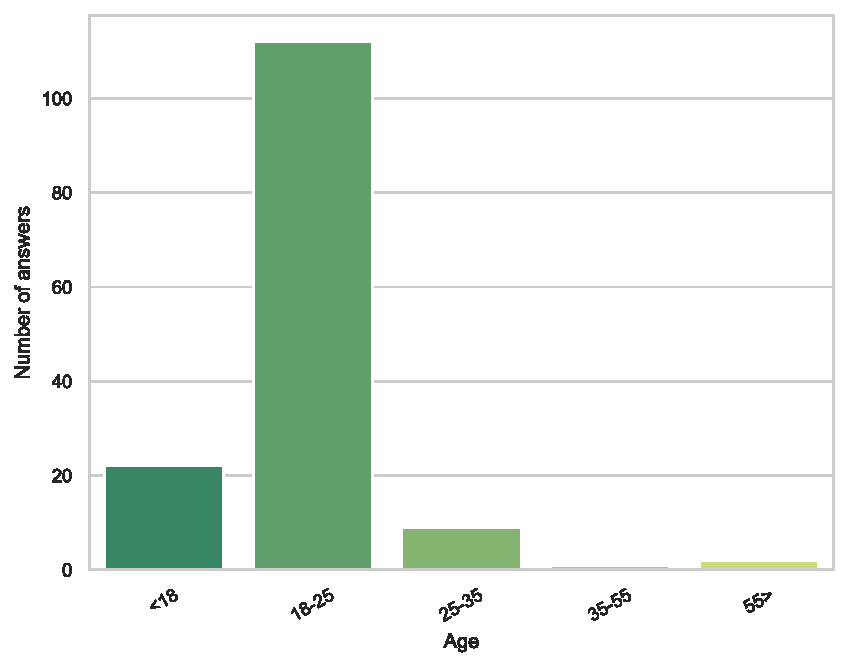
\includegraphics[width=.5\textwidth]{img/analysis/age_distribution.pdf}
	\caption{Age distribution of our respondents}
\end{figure}
The majority of our respondents are of ages $18 \mhyphen 25$, followed by a minority of users under 18 years. Those remaining are distributed across people aged
$25 \mhyphen 35$ and $>55$, with no respondent of age $35 \mhyphen 55$.

About the main province in which the respondents take public transport:
\begin{figure}[H]
	\centering
	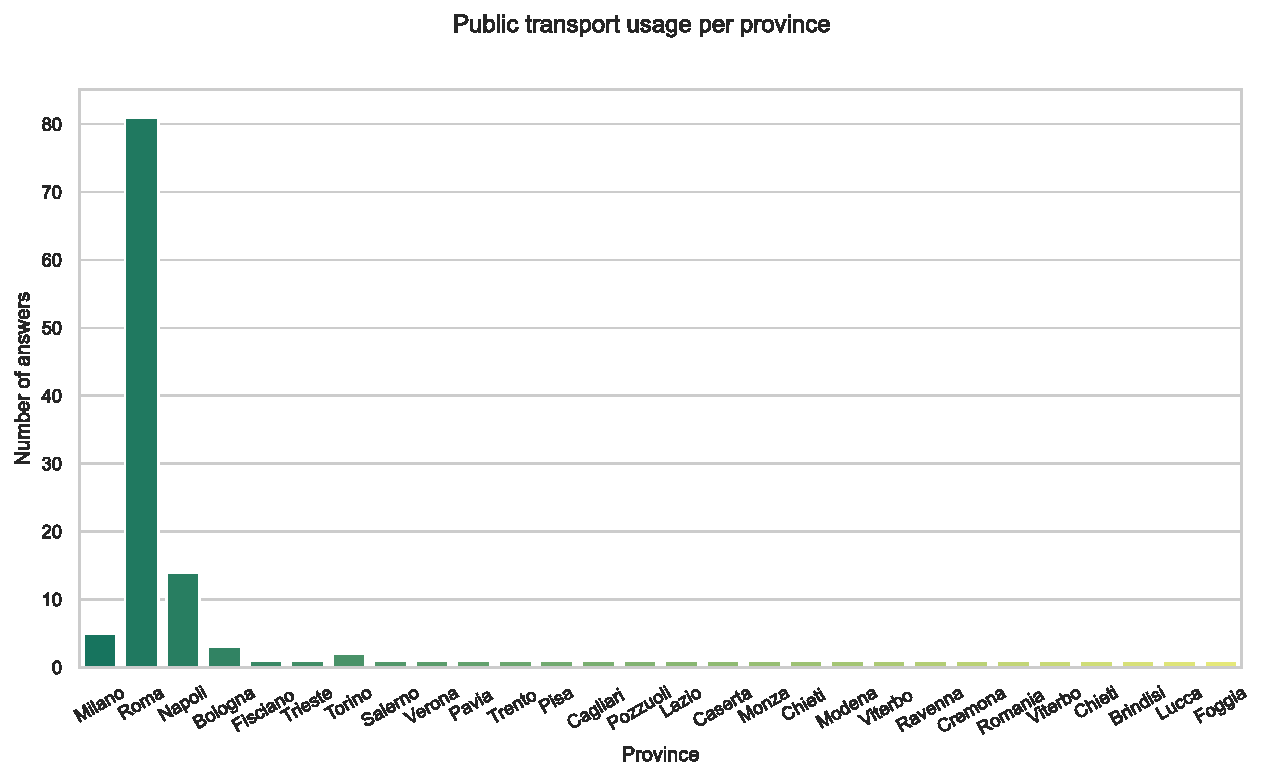
\includegraphics[width=.8\textwidth]{img/analysis/public_transport_usage_per_province.pdf}
	\caption{Public transport usage per province}
\end{figure}
As we can see, the majority uses public transport in Rome, with a minority in Milan and Naples. These results were obtained after having modified
the questionnaire. As explained above, initially, we were asking for the city and not the province.

We are also interested in the most used operating system among the respondents:
\begin{figure}[H]
	\centering
	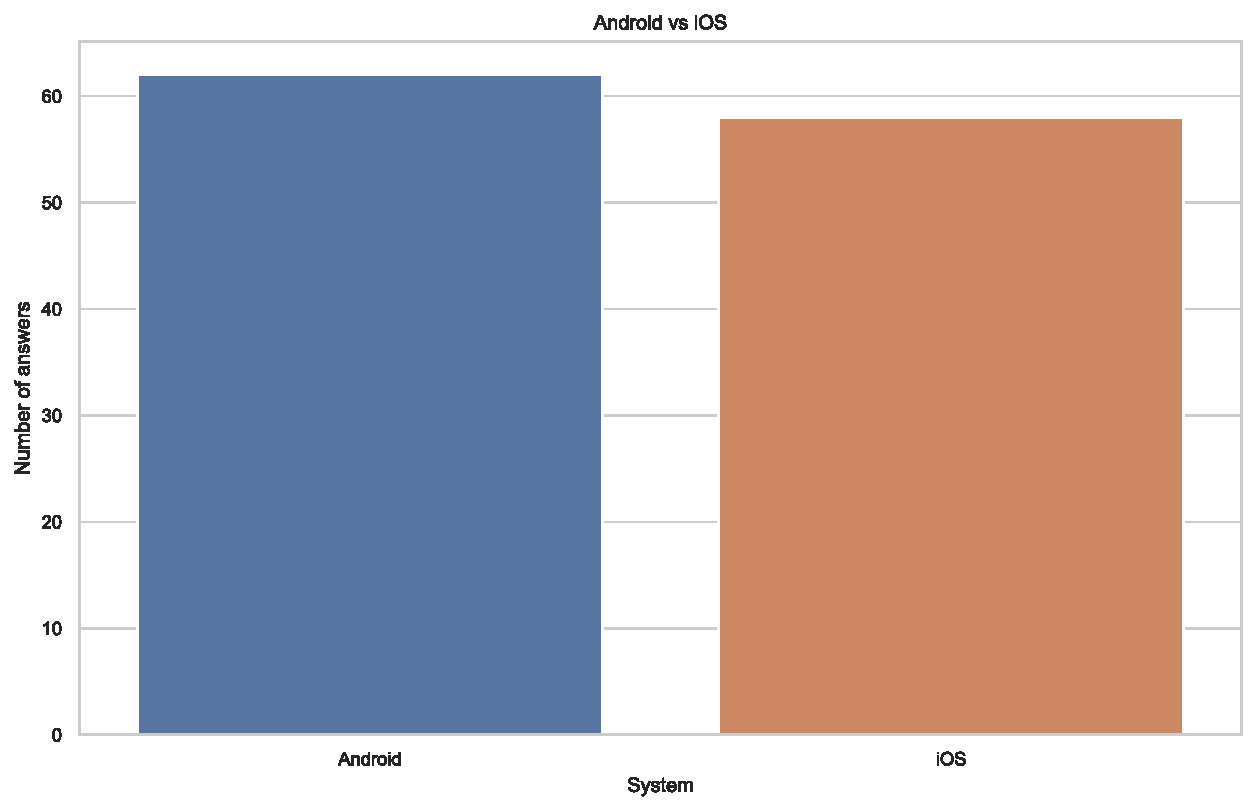
\includegraphics[width=.5\textwidth]{img/analysis/android_v_ios.pdf}
	\caption{Android VS iOS}
\end{figure}

Hoping for a more noticeable difference, the statistic shows that the obtained results are similar: 52\% Android users and 48\% iOS users.
We have decided to implement an Android application.

As follows, we show the number of public transport users by their device's operating system
\begin{figure}[H]
	\centering
	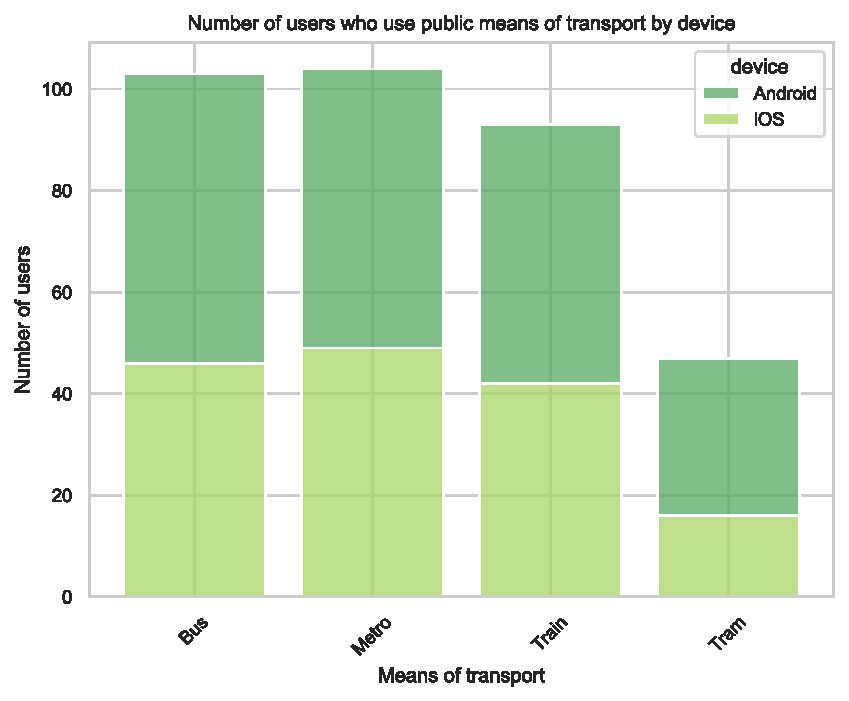
\includegraphics[width=.5\textwidth]{img/analysis/users_by_means_of_transport_by_device.pdf}
	\caption{Users by means of transport by device}
\end{figure}


Let's look at the number of public transport users by province:
\begin{figure}[H]
	\centering
	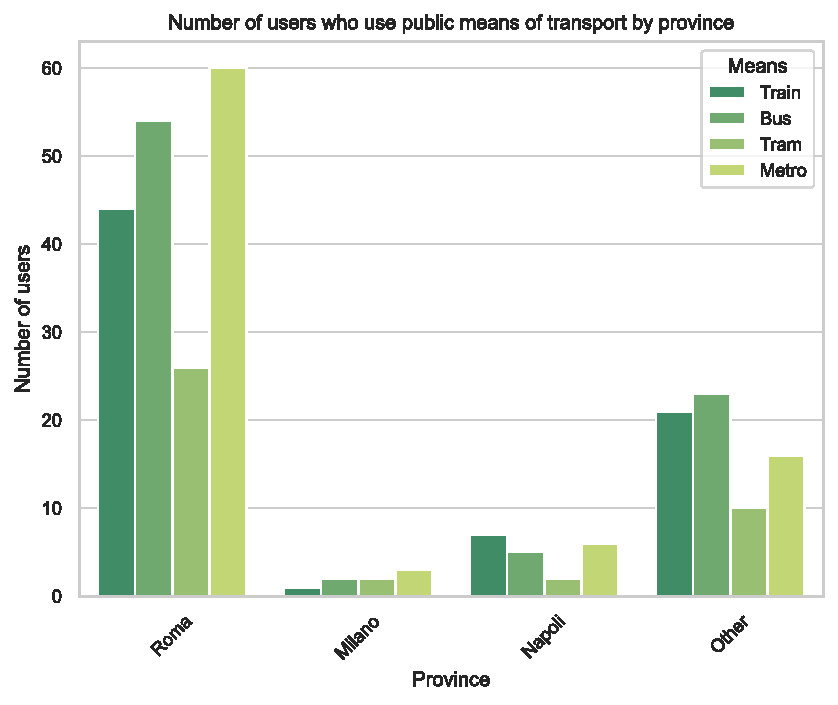
\includegraphics[width=.5\textwidth]{img/analysis/users_by_means_of_transport_by_province.pdf}
	\caption{Users by means of transport by province}
\end{figure}
Since the majority of the respondents use public transport in Rome, Naples and Milan, we have collected the statistics of other provinces in the `Other' column.
It is evident that, in each province, users take the metro and the bus mostly.

At the basis of our reasoning, the most frequent disservices caused by public transport are:
\begin{figure}[H]
	\centering
	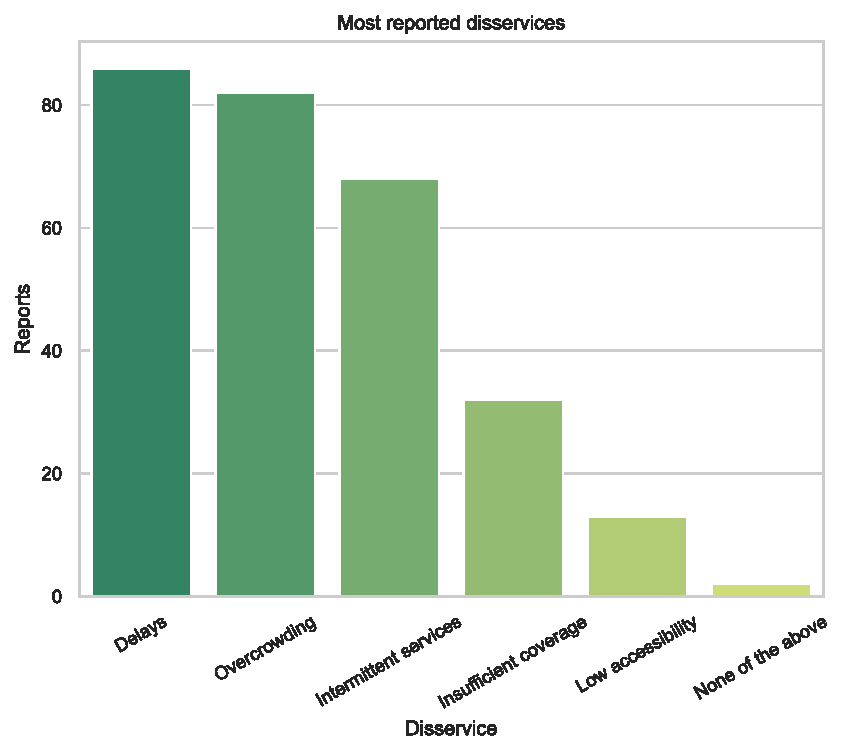
\includegraphics[width=.5\textwidth]{img/analysis/disservices_reports.pdf}
	\caption{Disservices reports}
\end{figure}
This analysis is fundamental to our project. It highlights the most frustrating aspects of public transport.
Those are the ones on which we should focus, in order to improve people's experience while using public transport.
As shown, the majority of the respondents report about delays and overcrowding. The obtained results give us a further confirmation of our objective.


In the form, we ask some questions in order to understand users preferences and how they would be interested 
in our idea. 
Crowdsourcing is at the basis of our application. Retrieving information, about possible delays or 
transport overcrowding, directly from the community of users will make transportation more efficient. 
But, are users willing to partecipate? If so, would they be more incentivized having some kind of reward (e.g. charity,features and customization unlocking)?
Let's look at some statistics 
\begin{figure}[H]
	\centering
	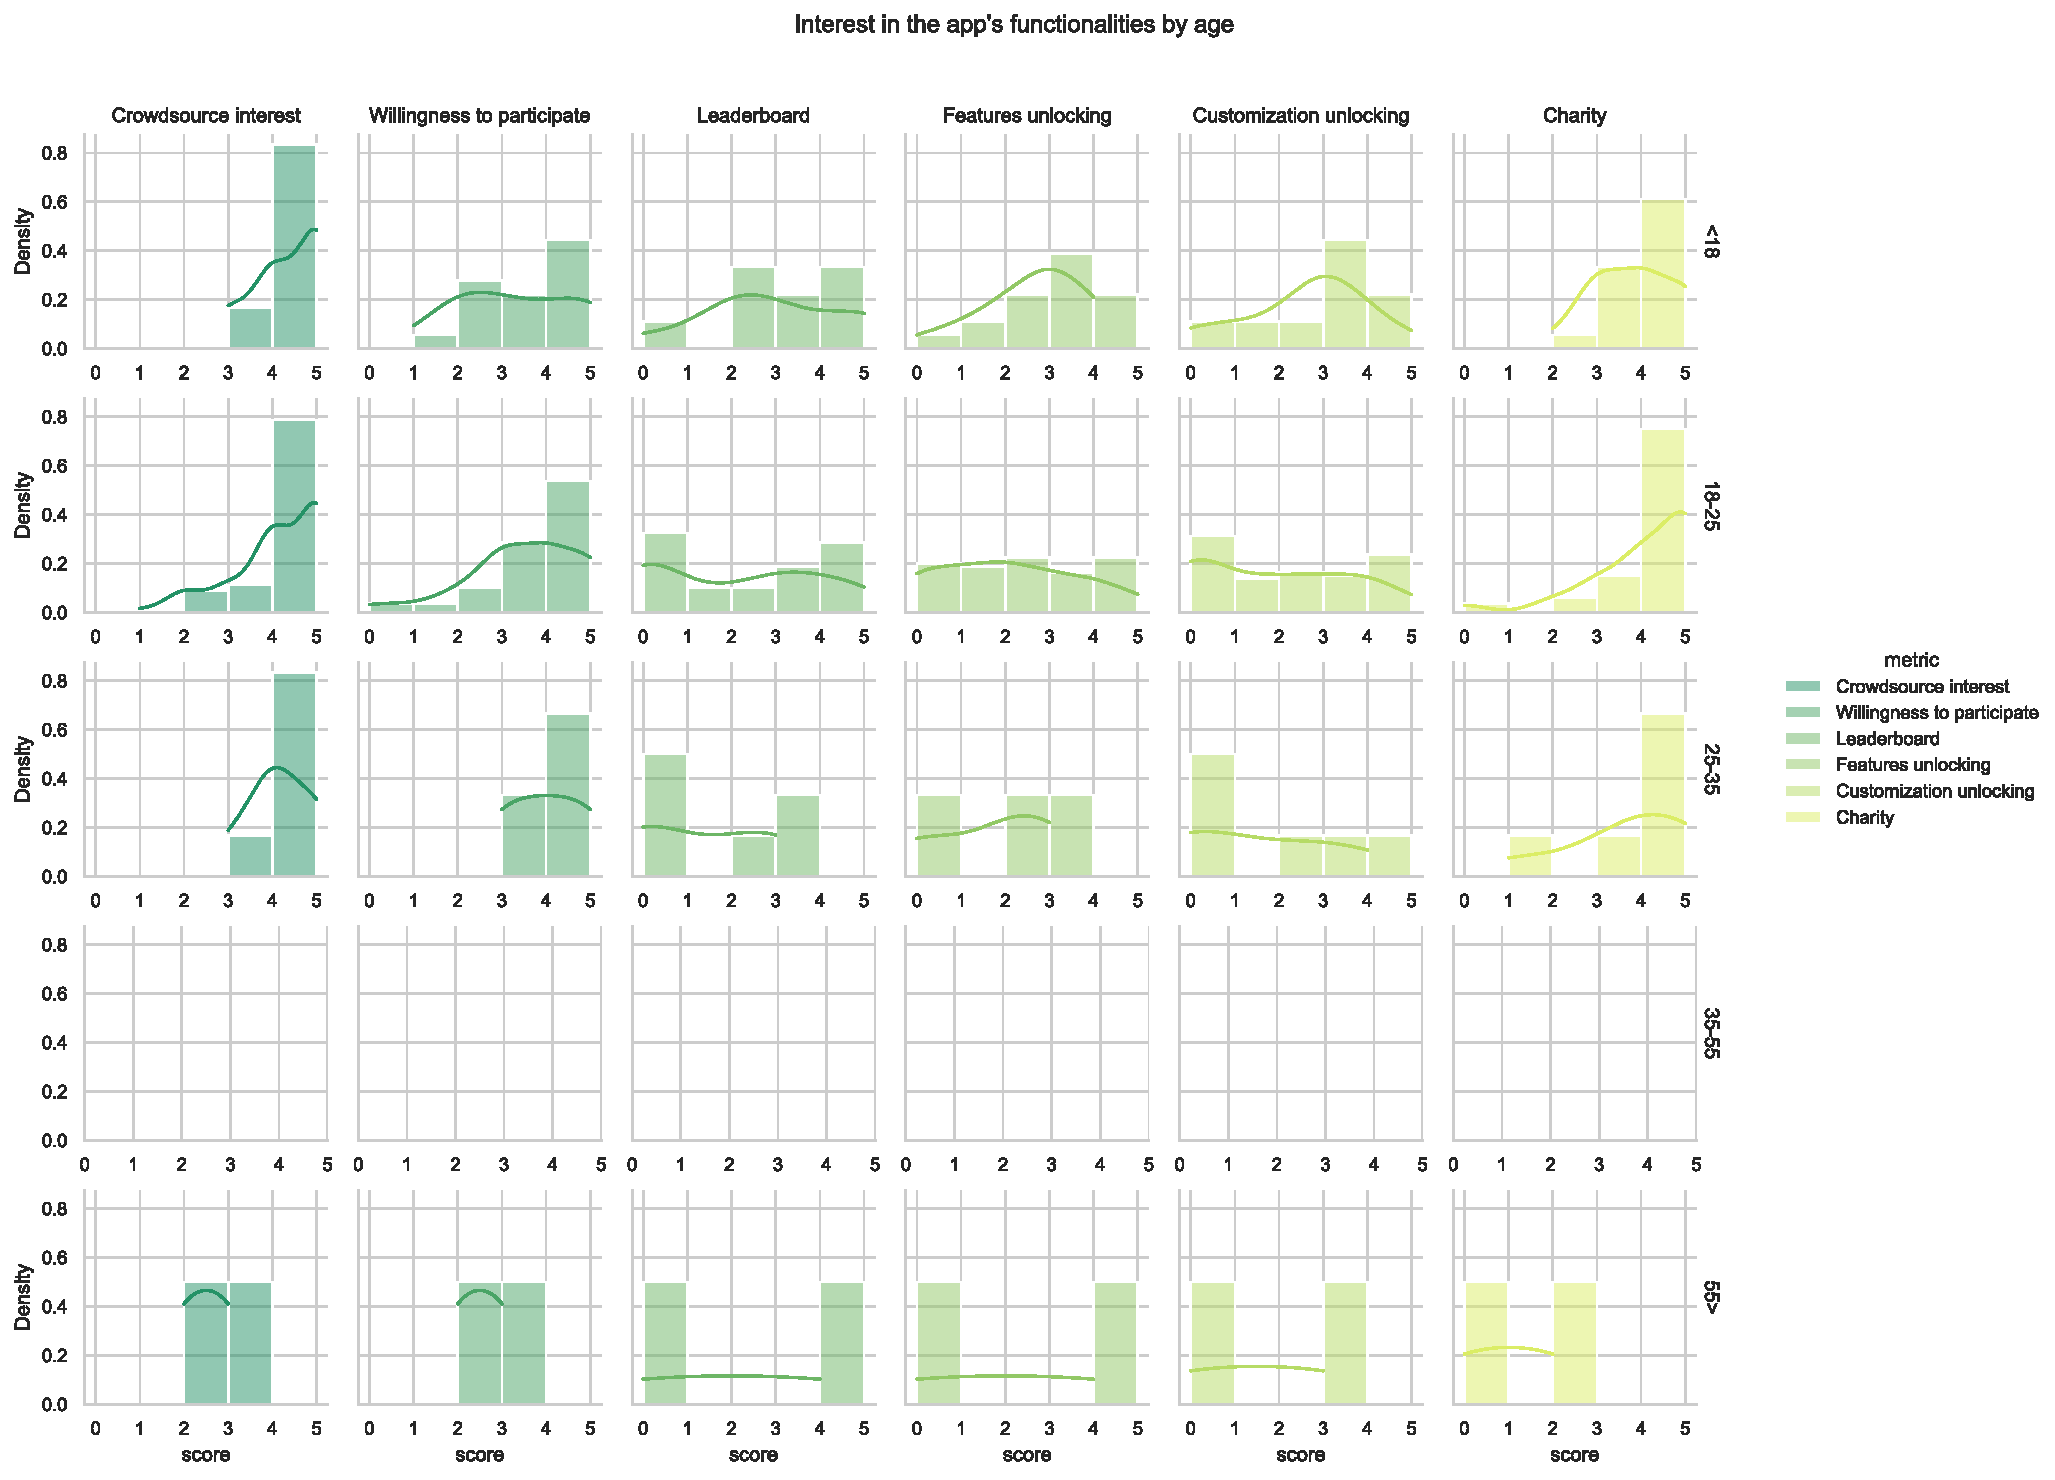
\includegraphics[width=.5\textwidth]{img/analysis/interest_app_functionalities.pdf}
	\caption{Interest app functionalities}
\end{figure}
The graphic above shows the various preferences by age. 


Since the majority of the respondents are of ages $18 \mhyphen 25$, let's look at their statistics deeply:  
\begin{figure}[H]
	\centering
	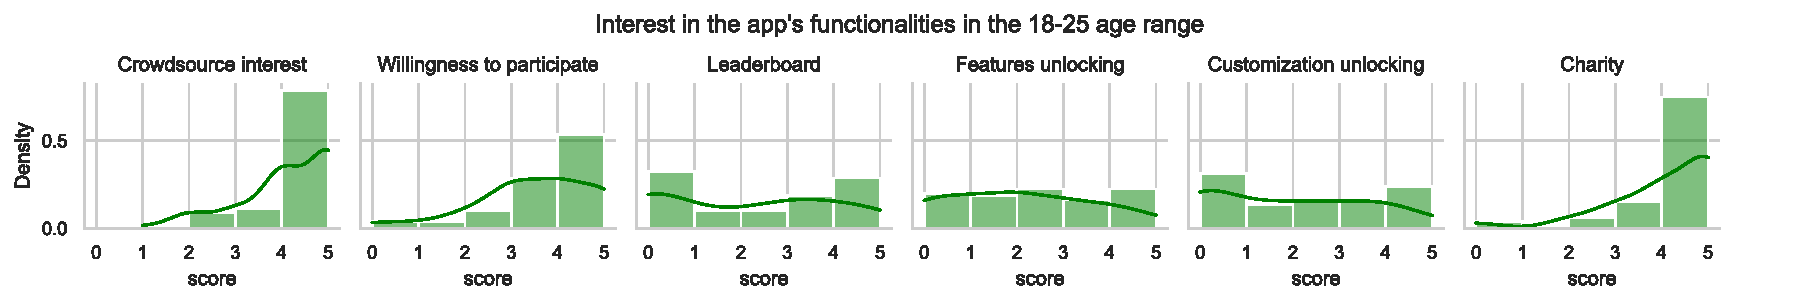
\includegraphics[width=.9\textwidth]{img/analysis/interest_app_functionalities_18_25.pdf}
	\caption{Interest app functionalities $18 \mhyphen 25$}
\end{figure}

Being more specific, without considering the age of the respondents 
\begin{figure}[H]
	\centering
	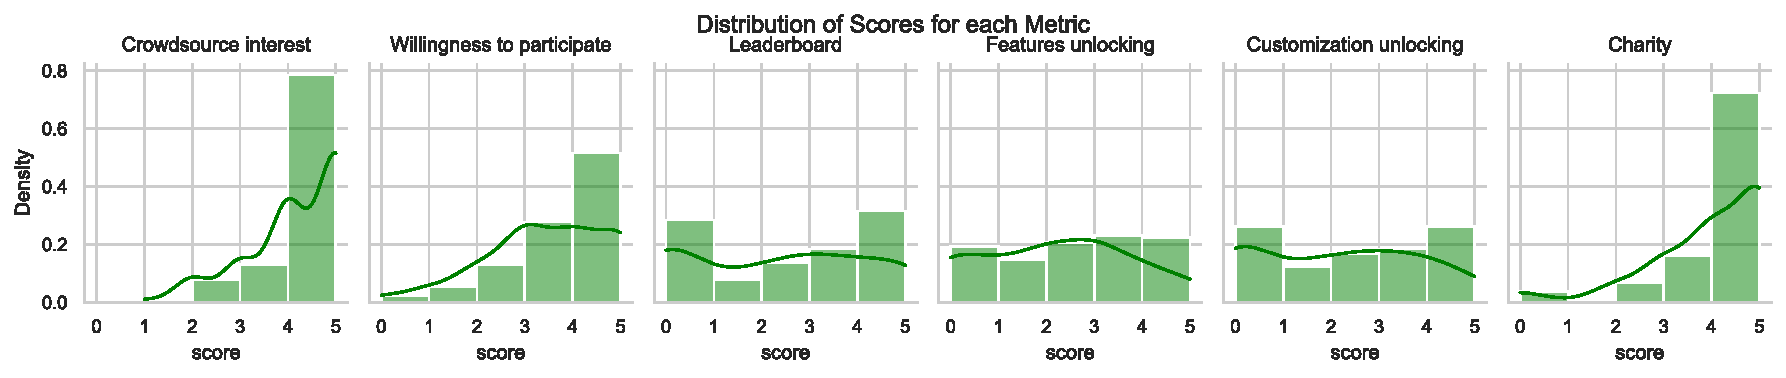
\includegraphics[width=.9\textwidth]{img/analysis/distribution_of_scores_for_each_metric.pdf}
	\caption{Distribution of scores for each metric}
\end{figure}

For each metric,a violinplot, with the distribution of the scores for each age group, is shown 
\begin{figure}[H]
	\centering
	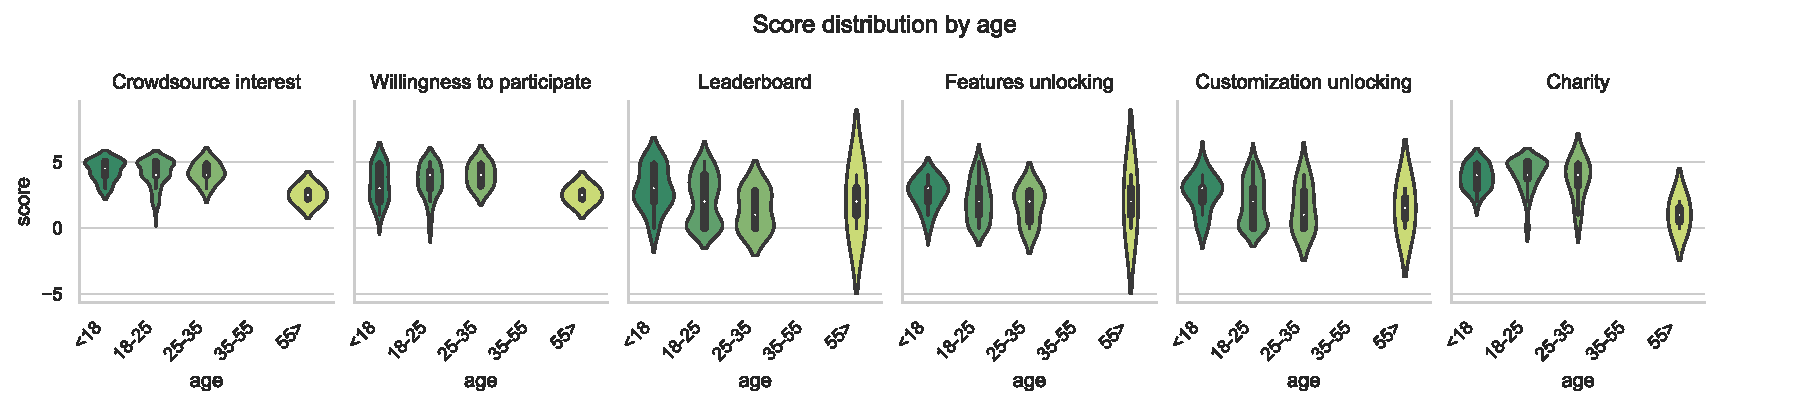
\includegraphics[width=.9\textwidth]{img/analysis/score_distribution_by_age.pdf}
	\caption{Score distribution by age}
\end{figure}

Now, let's look at numbers! 
\begin{figure}[H]
	\centering
	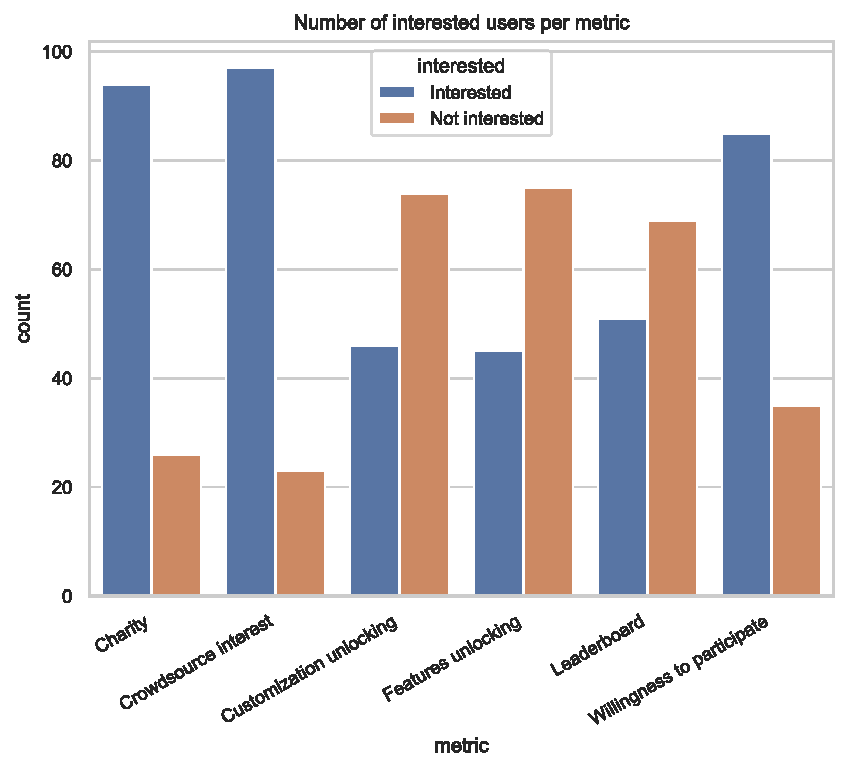
\includegraphics[width=.5\textwidth]{img/analysis/interested_users_per_metric.pdf}
	\caption{Interested users per metric}
\end{figure}
As we can see, the majority is not interested in a leaderboard of the users who have reported the greatest number of 
information (e.g. delays, overcrowding). As reward systems, features and costumization unlocking have not captured the attention of the 
respondents. However, their crowdsource interest and willingness to partecipate in such a community give us a positive feedback. 
Chiarity donations incentivize them more. 


\section{Storyboarding}\label{sec:storyboarding}

\paragraph{Tasks}

After our questionnaires, we wanted to clearly identify a set of \emph{core} tasks that should be
supported by the application.

\begin{titlebox}[The Tasks:]
	\begin{itemize}\label{list:tasks}
		\item Reporting public transport delays to other users
		\item Reporting overcrowding in a public transport to other users
		\item Spending points for a donation to a non-profit organization
		\item Looking for a route to a destination
	\end{itemize}
\end{titlebox}


For each of those we then proceeded to produce a storyboard detailing the sequence of
interactions that a user must perform in order to complete the task.


\begin{figure}[H]
	\centering	
	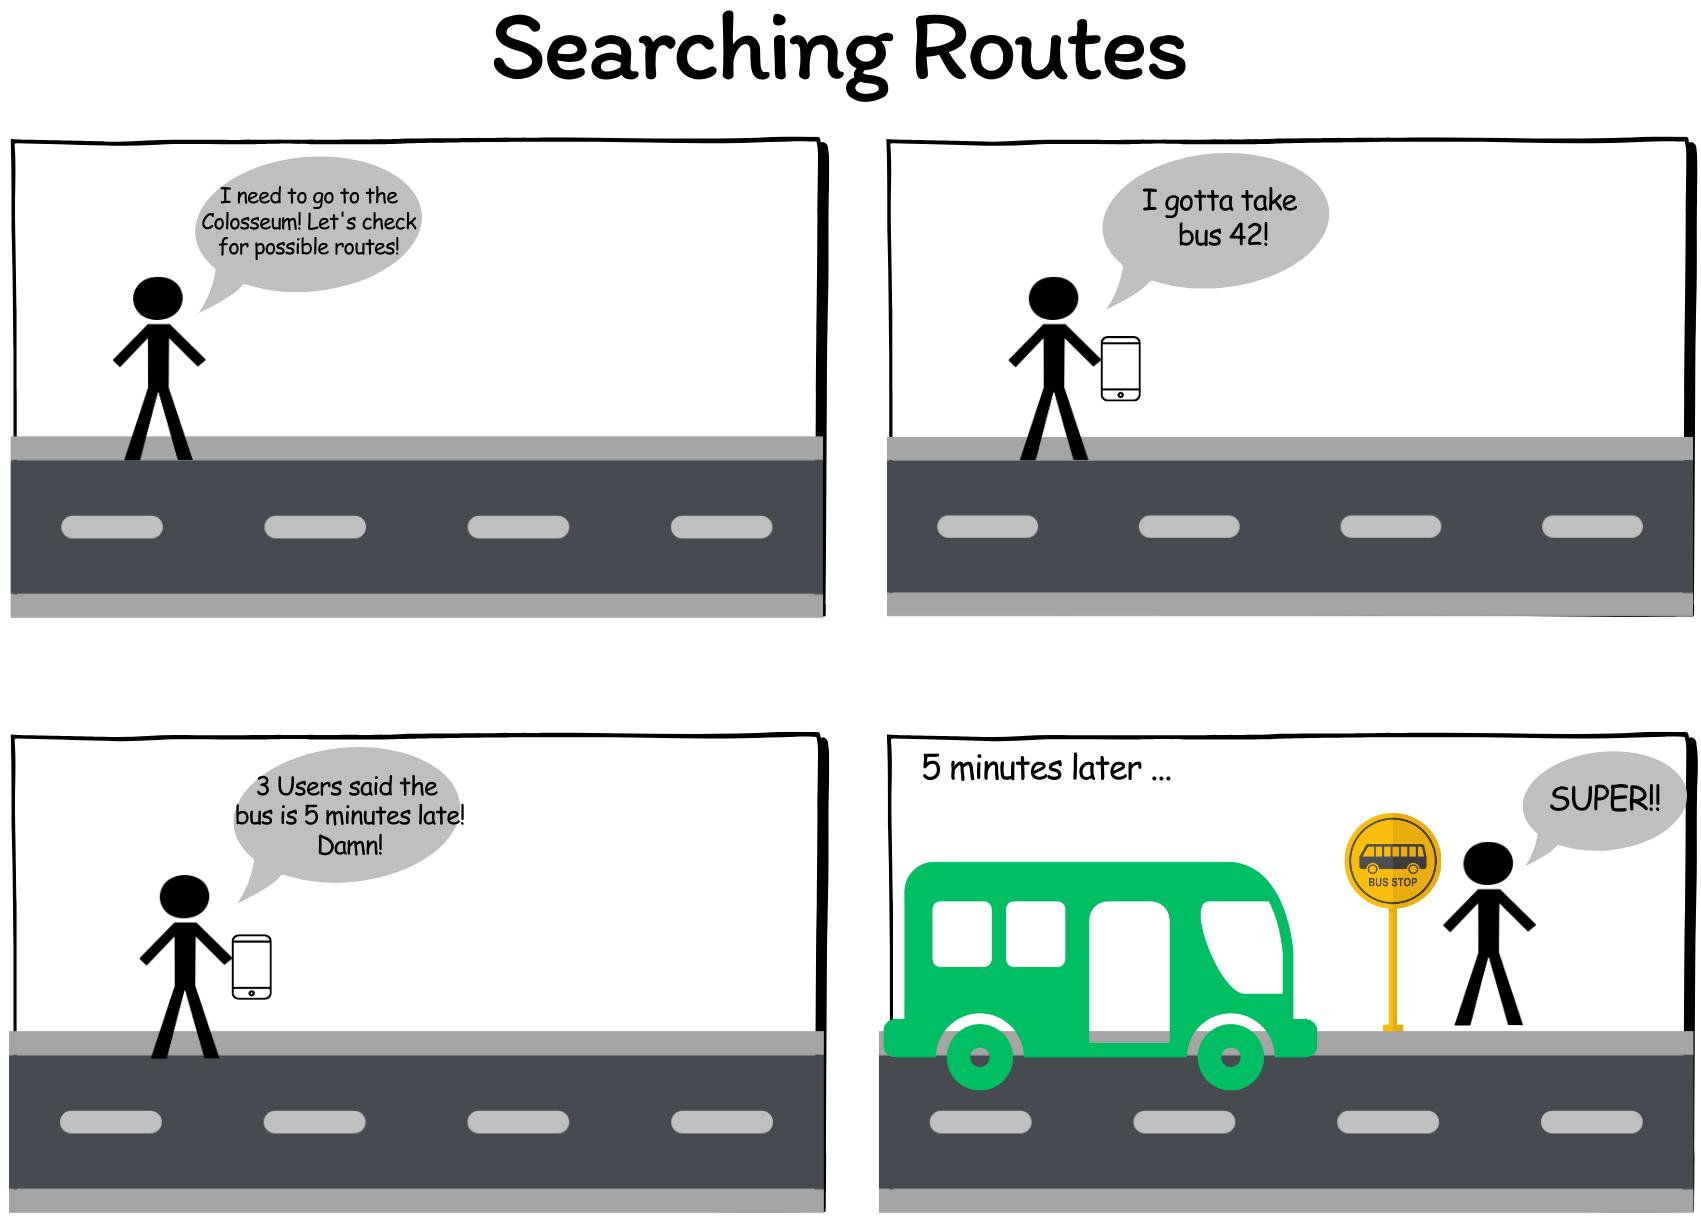
\includegraphics[width=.5\textwidth]{img/storyboards/storyboard_searching_routes.png}
	\caption{Searching for routes}
	\label{fig:a}
\end{figure}	
\textbf{Scenario Description:} Imagine being a tourist trying to reach Colosseum,
 due to the ZTL the car is out of the question. So you want to find the fastest
  path to reach your destination. Thus you open our app to find the route to be followed and any reported delays.    \\
\textbf{Task Description:} Open the app, type your destination point,
 and find the available routes. For every available route, you will also find any certified delays
 reported by one or more users.\\
\begin{figure}[H]	 
	\centering
	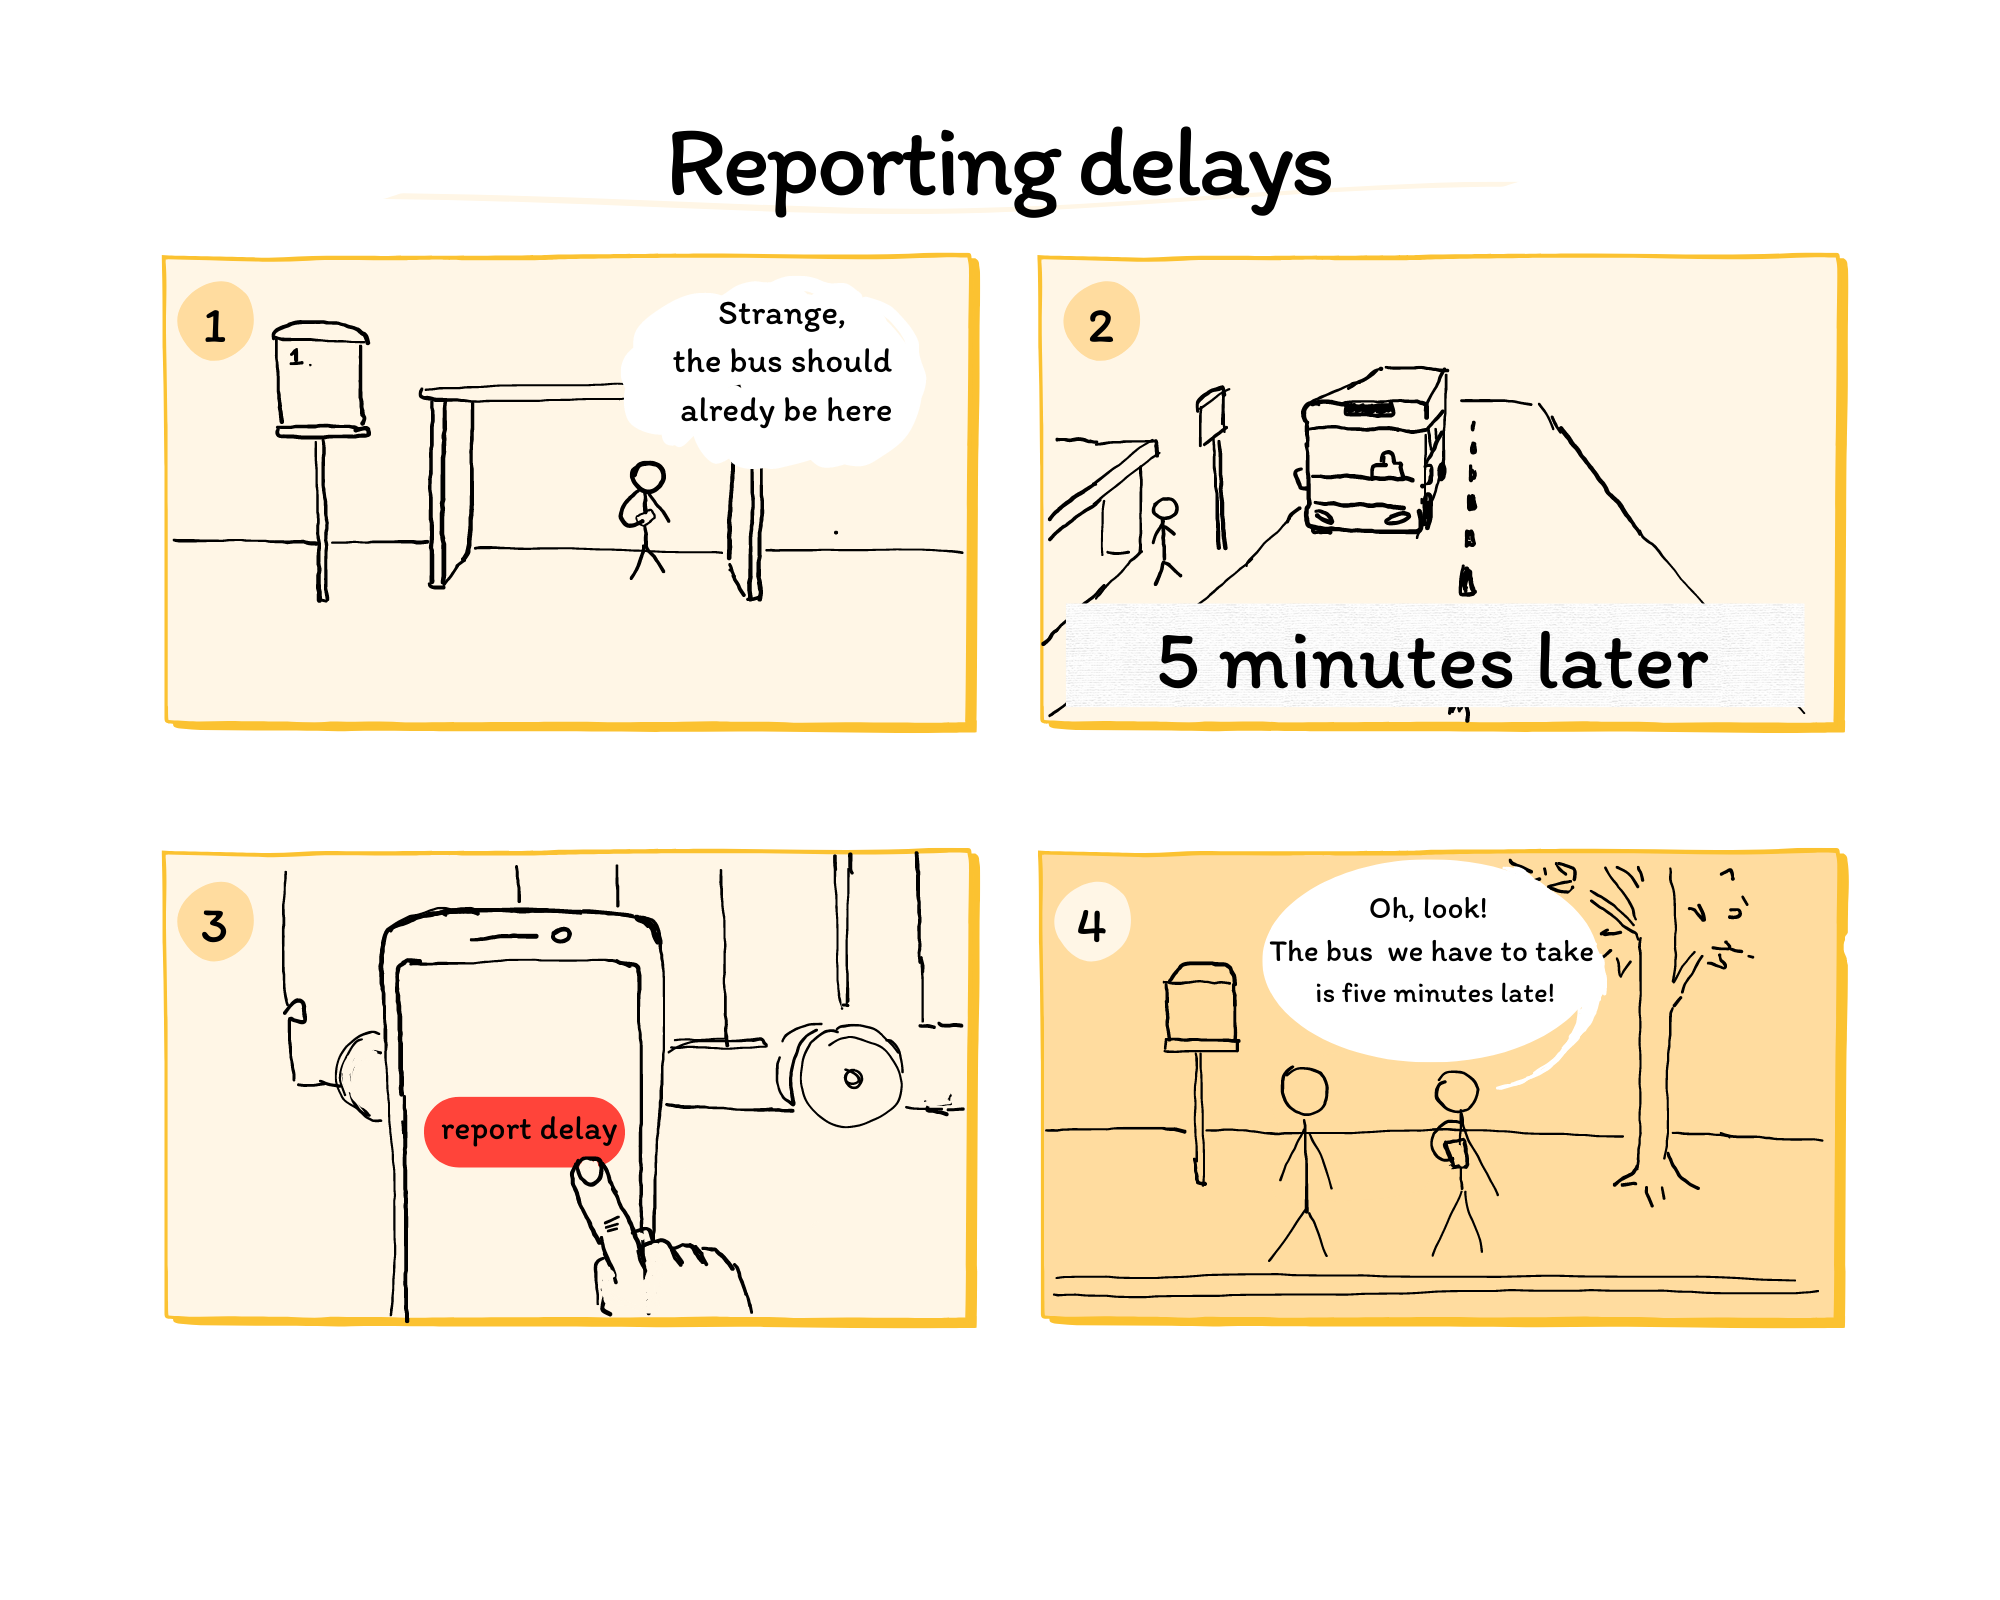
\includegraphics [width=.5\textwidth]{img/storyboards/storyboard_reporting_delays.png}
	\caption{Reporting Delays}
	\label{fig:b}
\end{figure}

\textbf{Scenario Description:} Imagine that you have been waiting
for a bus in the center of Rome for 10 minutes. Your mobility application tells you
 that the next bus should have already passed two minutes ago.
  Thus when the bus passes, you can inform the app of the real timing and it will recalculate the actual
   delay based on your personal experience.    \\
\textbf{Task Description:} Open the app, type the bus you are taking, and click the proper button
 to report the actual time at which you got on the bus and this, as a consequence,
  will inform the other users of any possible delay.\\

\begin{figure}[H]
	\centering	 
	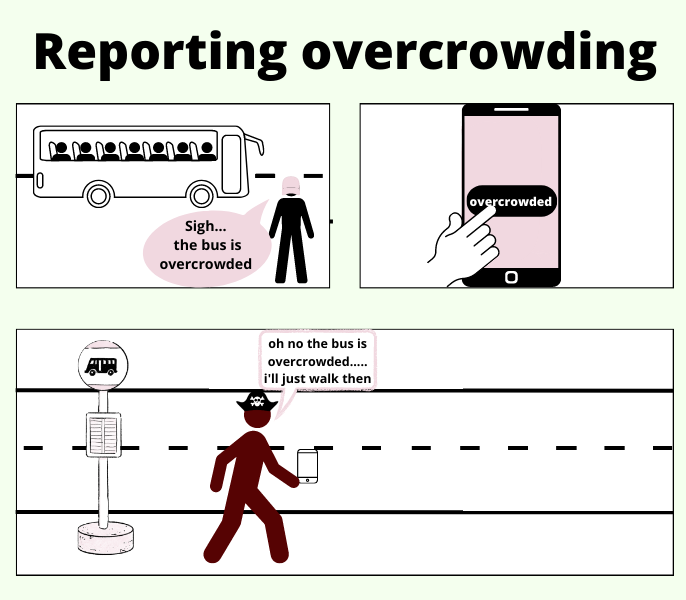
\includegraphics[width=.5\textwidth]{img/storyboards/storyboard_overcrowding.png}
	\caption{Reporting Overcrowding }
	\label{fig:c}
\end{figure}
\textbf{Scenario Description:} Imagine that you are willing to take a bus in the center of Rome,
 you know that it may be full, thus your waiting time may be longer than the one you expected. When the bus arrives,
  you may check if it is too full to enter and you may report it to the other users, who may benefit from this information.\\
\textbf{Task Description:} Open the app, and use the button to report that the bus you are taking is overcrowded.
 The other users will have this information reported near the one on the waiting time of that bus.\\

\begin{figure}[H]
	\centering	
	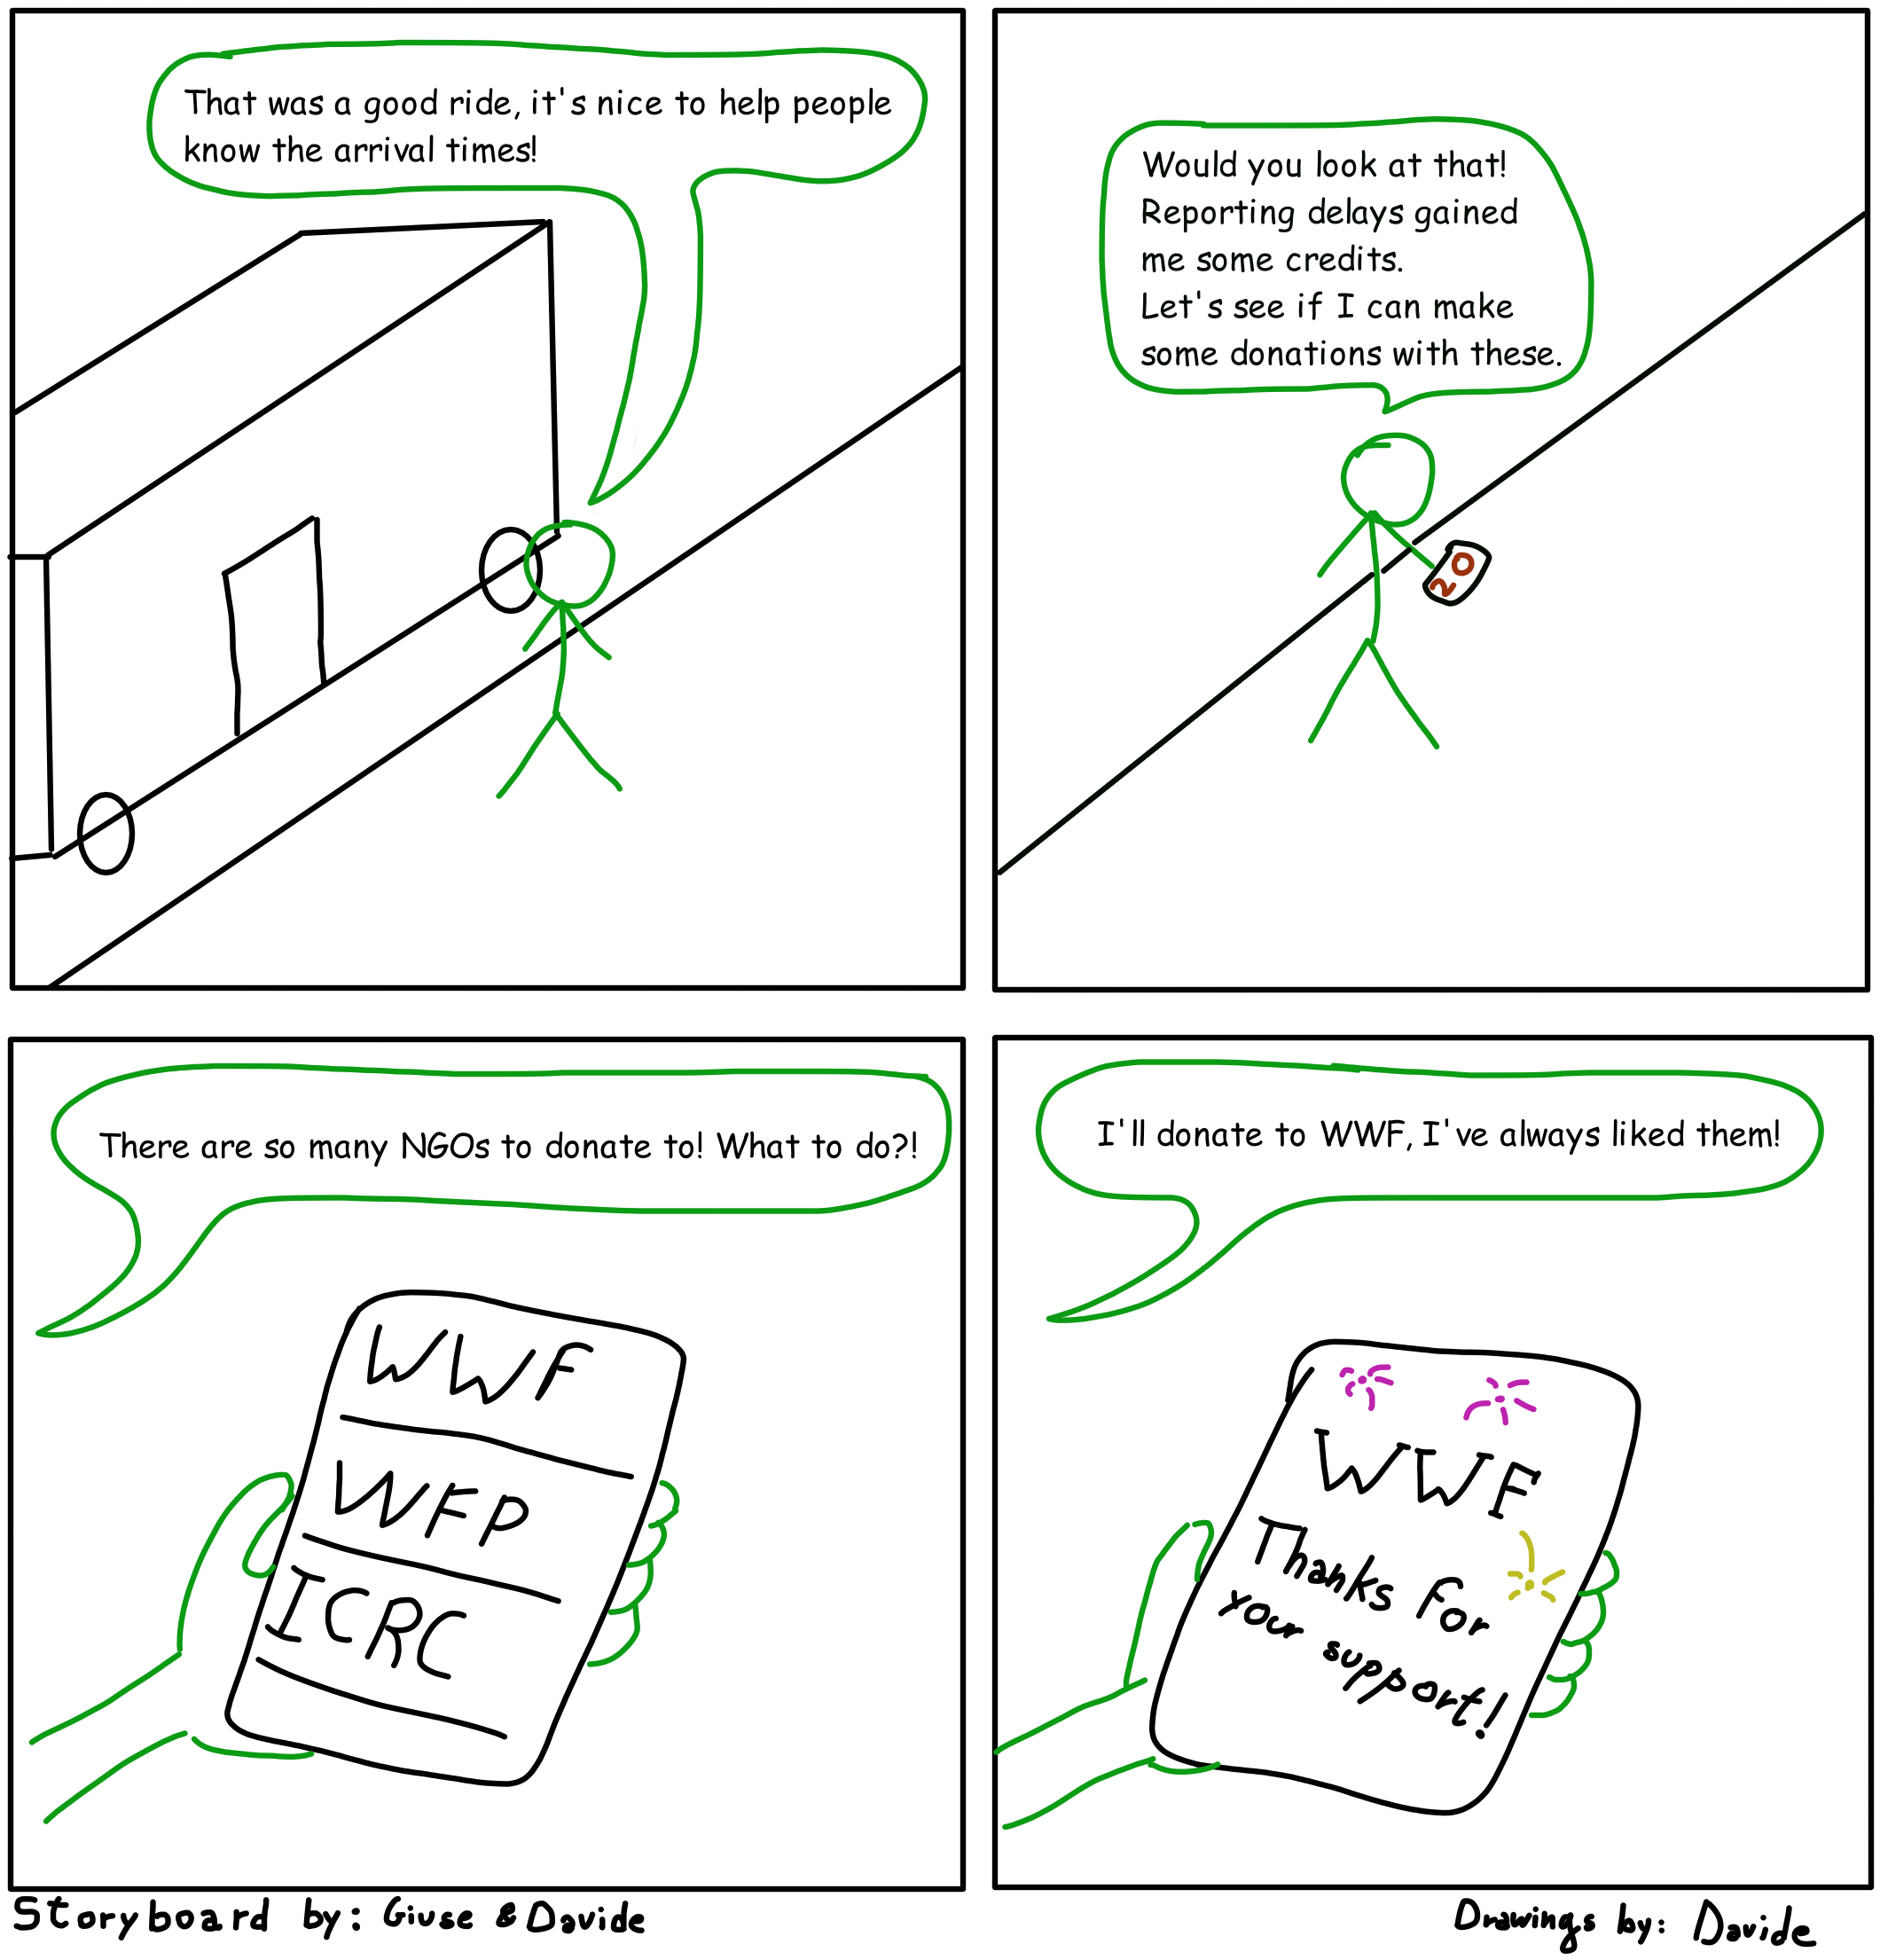
\includegraphics [width=.5\textwidth]{img/storyboards/storyboard_donations.png}
	\caption{Donating to a non-profit}
	\label{fig:d}
\end{figure}
\textbf{Scenario Description:} Imagine that for every departure reported, you get to store a certain amount of credits.
 After x report, you can devolve your credits into charity in one of the NGOs chosen by the user, 
 among those proposed by the application. Thus every free contribution to the application service
  leads to the help of other people in need.\\
\textbf{Task Description:} Open the app, check on your profile the number of accumulated credits
 (and the respective correspondence in the local currency), open the page with the list of charity options,
  and choose the one you prefer.\\

\end{document}